\setchapterpreamble[u]{\margintoc}
\chapter{Neutrinos in IceCube} \labch{nu_icecube}

% Ever since the discovery of neutrino by Cowans and Reines \sidecite{nu_discovery},significant advancements have been made in detector technologies.
% These include the radiochemical detection of MeV-scale neutrinos produced by nuclear fusion in the Sun \sidecite{solarneutrinos}, and the detection of higher energy atmospheric neutrinos in deep underground telescopes \sidecite{ACHAR1965196,PhysRevLett.15.429}.
% The observation of neutrinos from supernova 1987a \sidecite{SN1987A_Baksan,SN1987A_superK,SN1987A_IMB} marked a significant milestone in astronomical research as it was the first-ever observation of such an event through these messengers, thereby opening a new window in the field of astronomy. \par

The birth of neutrino astronomy has led to the development of specific neutrino telescopes designed to explore the cosmos using these elusive particles. 
This chapter introduces the IceCube Neutrino Observatory, an advanced detector whose data forms the basis of the analysis discussed in this thesis. 
Later sections will explore different types of neutrino interactions and explain how experiments like IceCube can be used to detect the particle products of these interactions.\par 

\section{Detection of Neutrinos} 
\label{sec:nu_detection}

\subsection{Neutrino-Nucleaon Deep Inelastic Scattering}
\subsection{Energy losses of Particles in ice}
\subsection{Cherenkov Radiations}



\section{IceCube Neutrino Observatory}
\label{IC_detector}
As described in \ref{sec:nu_detection},the detection of high-energy neutrinos requires a large detector due to their small interaction cross-section. When these neutrinos interact, they produce Cherenkov photons which are produced due to the passage of charged daughter particles. Therefore, the detector must be transparent to these photons. Such a large detector volume can be acquired by using natural resources such as large bodies of water or ice; by deploying photosensors underneath to create a sufficiently sized detector.\par
This concept was first introduced in 1960 \sidecite{Markov:1960vja}. The groundwork for implementing such a detector began with water-based experiments like DUMAND \sidecite{PhysRevD.42.3613}, which was planned to be deployed in the sea near the main island of Hawaii and another detector with a similar design Lake Baikal \sidecite{BELOLAPTIKOV1997263}. First ever large-scale neutrino telescope built was predecessor of IceCube experiment called AMANDA \sidecite{ANDRES20001} at the geographic South Pole. A few hundred optical modules were dropped under the ice sheet of this dry continent between the depth of 1.5 to 2 km. Needless to say, the IceCube detector, the largest neutrino telescope in the world today, benefitted greatly in terms of design and performance from all the research and development work that was done with AMANDA. 
There also exists a large volume water-based neutrino telescope in the Northern Hemisphere called ANTARES\sidecite{AGERON201111}, and its successor KM3NeT\sidecite{MARGIOTTA201483}, located in the Mediterranean Sea.\par
The following subsections will discuss various detector and hardware components of the IceCube detector. Additionally, the last section will cover the optical properties of the South Pole ice, as these properties strongly affect the analysis observable and therefore influence the flavor measurements presented in this thesis.\par

\subsection{Detector}
\begin{figure}
	\centering 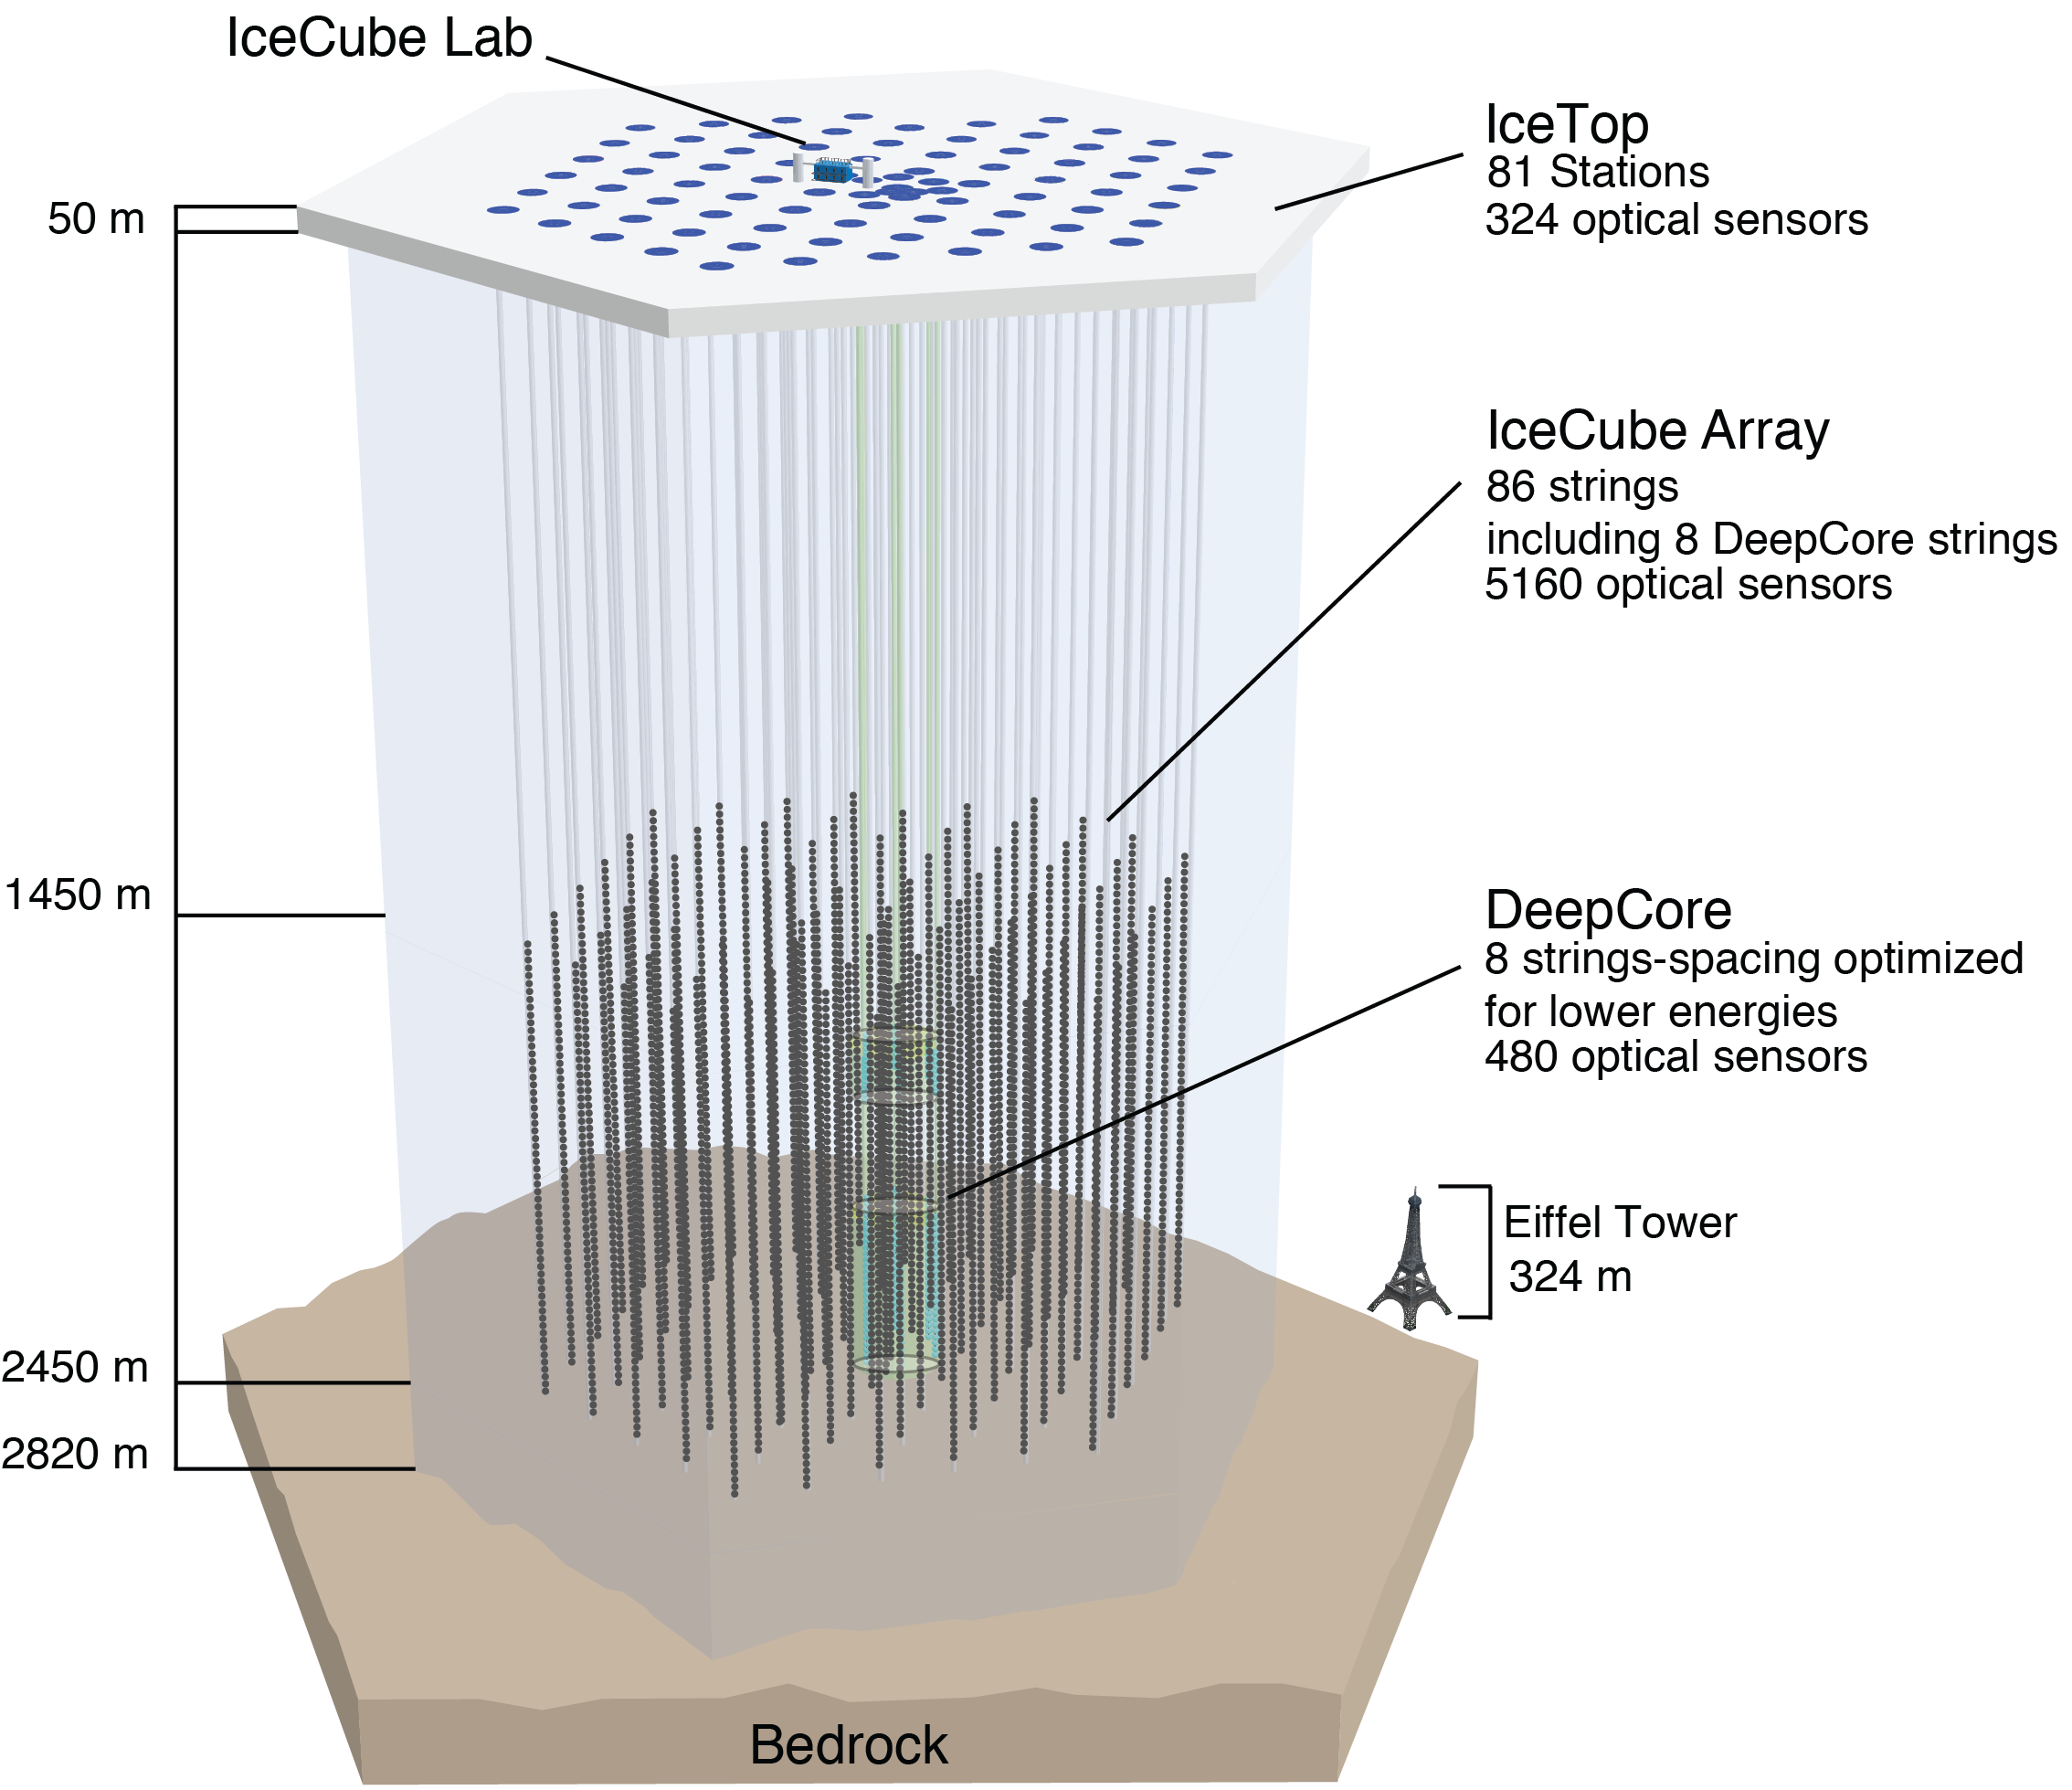
\includegraphics{./figures/nu_in_icecube/IceCubeArray_slim.png}
	\caption{A schematic overview of the IceCube detector and its components \cite{Aartsen_2017}}
    \labfig{ic_detector}
\end{figure}
    
\begin{marginfigure}
	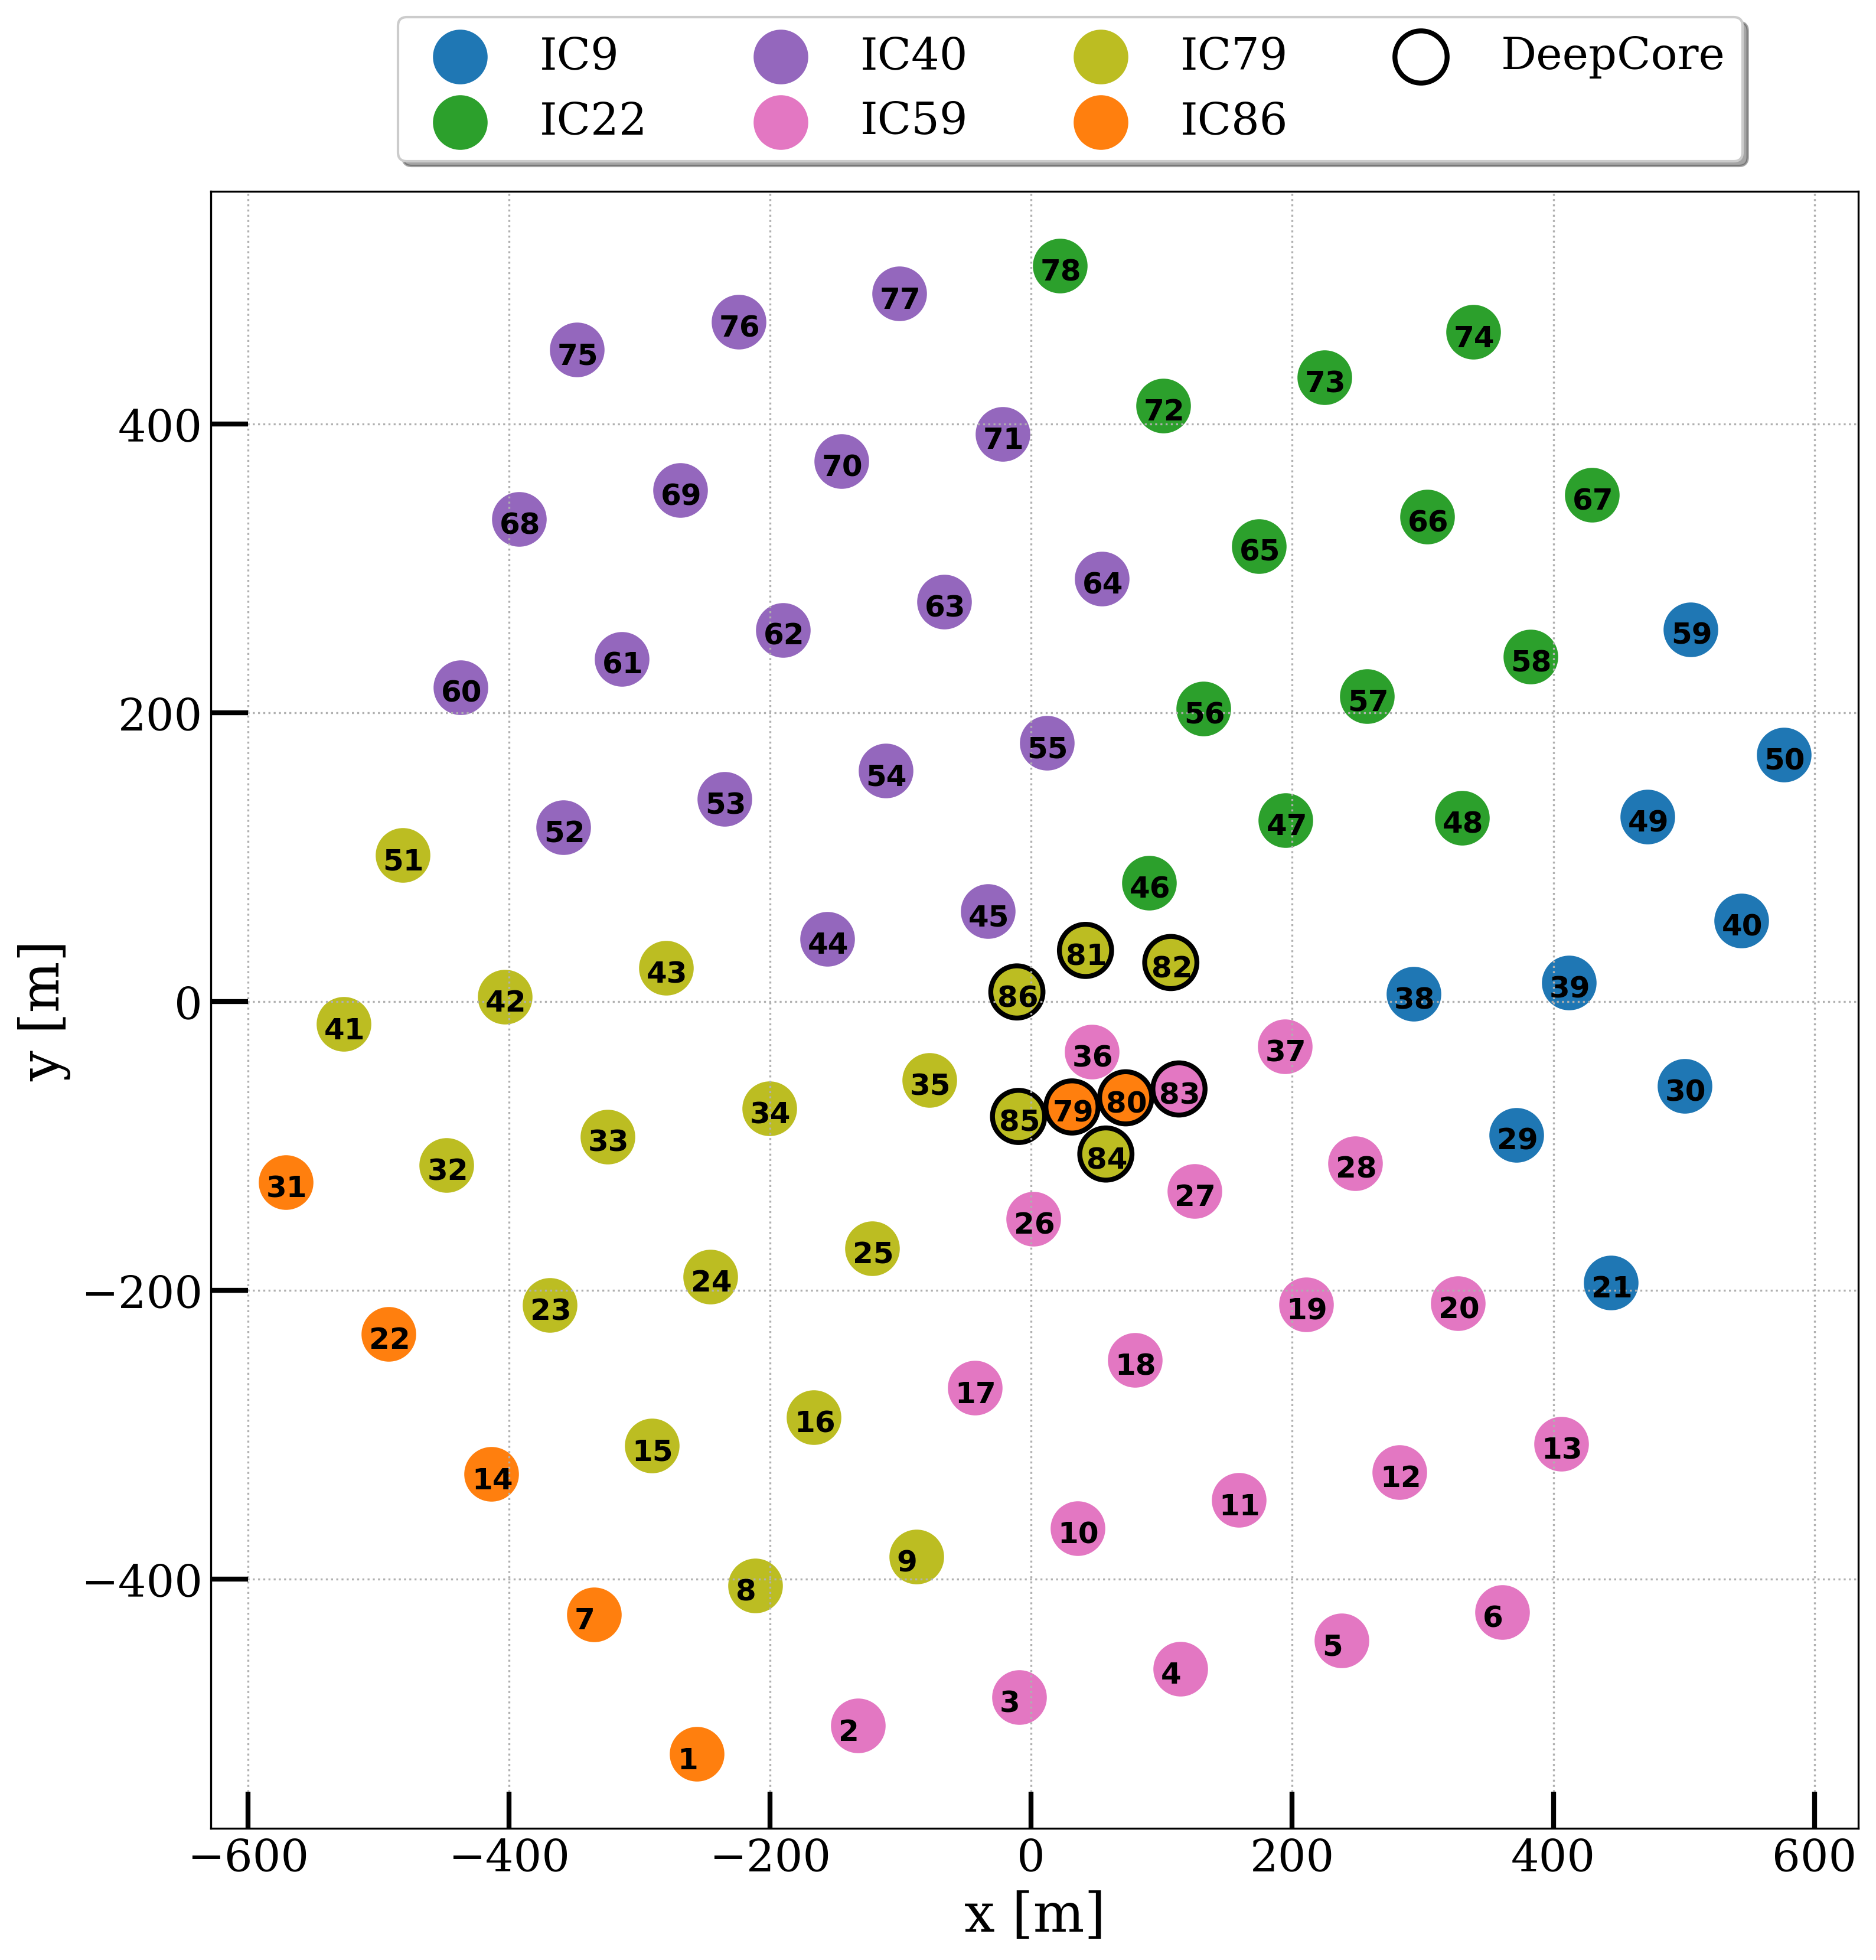
\includegraphics{./figures/nu_in_icecube/IC_Phase_Array.png}
	\caption{Top view of the location of each \emph{in-ice} strings of IceCube. Colour represents set of strings deployed in each seasons as described in \reftab{deployment_phases}. Note: IceTop Stations are not shown here.}
	\labfig{ic_phase_array}
\end{marginfigure}

\textbf{The IceCube Neutrino Observatory} is located at Amundsen-Scott South Pole Station at the geographic South Pole. It comprises a cubic kilometer of instrumented ice, equipped with 5,160 digital optical modules reffered as \emph{DOMs} from here-on (see \ref{sec:dom}), buried deep in the ice and 81 IceTop Stations on the surface of the ice, making itself the largest Neutrino Observatory in the world \sidecite{Aartsen_2017}. A schematic of the detector layout is shown in \reffig{ic_detector}. Four main components of the detector are \emph{in-ice array,DeepCore (inner extension of in-ice array),IceTop and IceCube Lab}. \par

\begin{description}
	\item[The Main \emph{in-ice} array] consists of 78 strings,\marginnote
    {\begin{kaobox}[title=\textbf{\emph{string} in IceCube}]
        An arrangement of DOMs attached on a twisted copper wire cable makes the so-called \emph{string} in IceCube.
    \end{kaobox}}
    each consisting of 60 DOMs, spaced vertically at a distance of 17 m between the depth of 1450 m to 2450 m under the ice sheet of Antarctica. Horizontal spacing between each of these strings is 125 m.  
	\item[\emph{DeepCore}] comprises inner 8 strings (see \reffig{ic_phase_array}) of the main\emph{in-ice} array, placed more closely together with horizontal string distance of 70 m and vertical DOM distance of 7 m \sidecite{deepcoredesign} between 1750 m to 2450 m depth. There's a region between depth of 1850 m to 2100 m, with no DOMs attached to the string as this region is the so-called \emph{dust layer} (see section \ref{sec:icemodel}), where optical scattering and absorprion is quite high and thus is not efficient to make reliable physics measurements. The Photomultipliers used in DOMs attached on these 7 strings also have higher Quantum Efficiency, which reduces the energy threshold to ~10 GeV. Although, IceCube's main goal is to detect astrophysical neutrinos, current topics of research spans much broader range (e.g fundamental properties of the neutrinos, such as oscillations \sidecite{Aartsen_2019_oscillations}, Physics beyond Standard Model searches such as Dark Matter \sidecite{Abbasi_2022} etc). 
	\item[\emph{IceTop}] is the surface detector array of the IceCube detector, primarily designed to detect Cosmic-ray airshowers and to be used as a veto layer for downgoing muons produced in these airshowers \sidecite{ABBASI2013188}. It consists of 81 \emph{stations} each having 2 tanks filled with clear ice (162 tanks in total). Each of these 162 tanks have 2 DOMs, similar to the ones deployed in \emph{in-ice} array, which makes it easier for both arrays to have a similar trigger and data acquistion system.
	\item[\emph{IceCube Lab}(ICL)] serves as the central operations' hub for the experiment, providing a crucial support for data acquisition and filtering. All the string cables connected to the aforementioned detcetor components are routed up to the ICL, from where triggered data is sent back to the northern hemispher via a satellite. Various other operations such as mainting the detector operations etc are also maintained from this building. 
	\end{description}

For the work presented in this thesis, neither \emph{deepcore} nor \emph{IceTop} data is used.
\begin{table}
    \caption{IceCube detector components deployed in each season (cumulative). Each configuration is represented as \emph{ICXX} where \emph{IC} stands for IceCube and \emph{XX} stands for number of total \emph{in-ice} strings at the end of that season}
    \labtab{deployment_phases}
    \begin{tabular}{cccc}
        \hline
        \hline
        Season & Configuration & Strings & IceTop Stations\\
        \hline
        2004-05 & IC1 & 1 & 4\\ 
        2005-06 & IC9 & 9 & 16\\ 
        2006-07 & IC22 & 22 & 26\\ 
        2007-08 & IC40 & 40 & 40\\ 
        2008-09 & IC59 & 59 & 59\\ 
        2009-10 & IC79 & 79 & 73\\ 
        2010-11 & IC86 & 86 & 81\\  
        \hline
        \hline
    \end{tabular}
    \end{table}


\marginnote{
    \begin{kaobox}[title=IceCube coordinates system]
        The IceCube coordinate system's origin is at 46500'E, 52200'N, 883.9 m elevation, which is quite close to centre of the \emph{in-ice} array. The y-axis points Grid North (toward Greenwich, UK), the x-axis points Grid East (90 degrees clockwise from North), and the z-axis points "up", forming a right-handed coordinate system.
    \end{kaobox}
    } 
The construction of the detector started taking place in 2005 and lasted for 7 Antarctic summer seasons till 2011 December. In each season, parts of the current day Hexagonal detector were deployed, as shown in \reffig{ic_phase_array} and numbers detailed in \reftab{deployment_phases}. A hot water drill was used to unfreeze the ice upto 2.5 km depth and 60 cm diameter into which these strings were then deployed (see \reffig{DOM_assembly}). The geometry of the detcetor, i.e The \emph{xy}-coordinates of the string were calculated from the drill tower position, surveyed during the deployment. Assuming the string was vertical, these coordinates were applied at all depths, with deviations of less than 1 m (later validated using the flasher data, see \ref{sec:DAQ}). Depths of the lowest DOM were determined from pressure readings, corrected for water compressibility and ambient air pressure, with vertical DOM spacings measured via laser ranger. All depths were converted to z-coordinates in the IceCube coordinate system \todo{Maybe draw a small schematic of coordinate system here next to the side note?}.\par  


\subsection{The Digital Optical Module (DOM)}
\label{sec:dom}
\textbf{The Digital Optical Module} (DOM) is a crucial component of the IceCube Neutrino Observatory, functioning as the heart of the detector. Each DOM is responsible for collecting the faint light signals produced by neutrino interactions in the Antarctic ice, amplifying these signals, and transmitting the data to the IceCube Lab \cite{Aartsen_2017}. From there, the data is relayed to the Northern Hemisphere via a satellite for further analysis. 

Inside each DOM, a 10-inch Photo Multiplier Tube (PMT) is positioned at the bottom, accompanied by essential circuitry for power conversion, data acquisition, calibration, control, and data transfer. Individual components of a DOM are as shown in \reffig{DOM_schematic}, functions of each of which is explained briefly below.
\begin{marginfigure}
    %\vspace*{-4.5cm}
    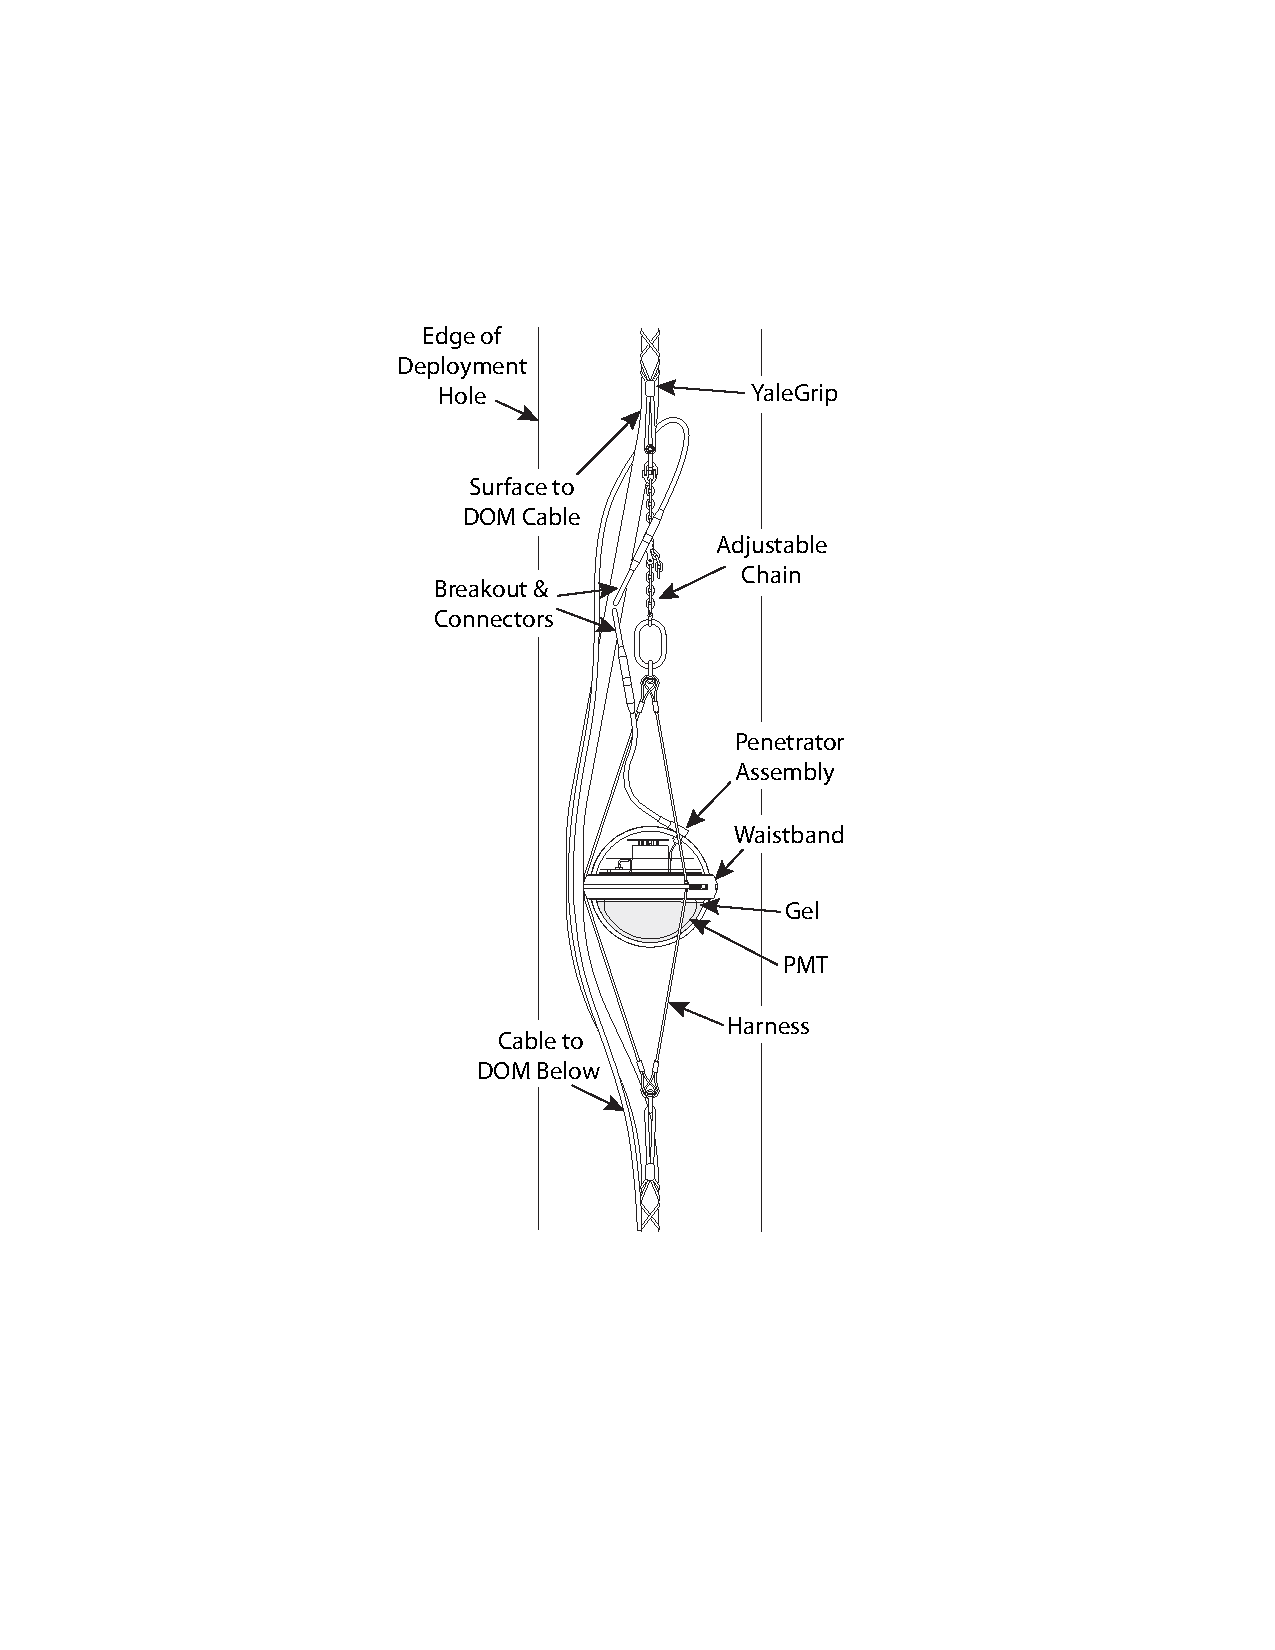
\includegraphics{./figures/nu_in_icecube/domfig2a-CableAssembly.pdf}
    \caption{A schematic of DOM CableAssembly being deployed in a water hole, created by hot water drill \cite{Aartsen_2017}.}
    \labfig{DOM_assembly}
\end{marginfigure}

\begin{marginfigure}
	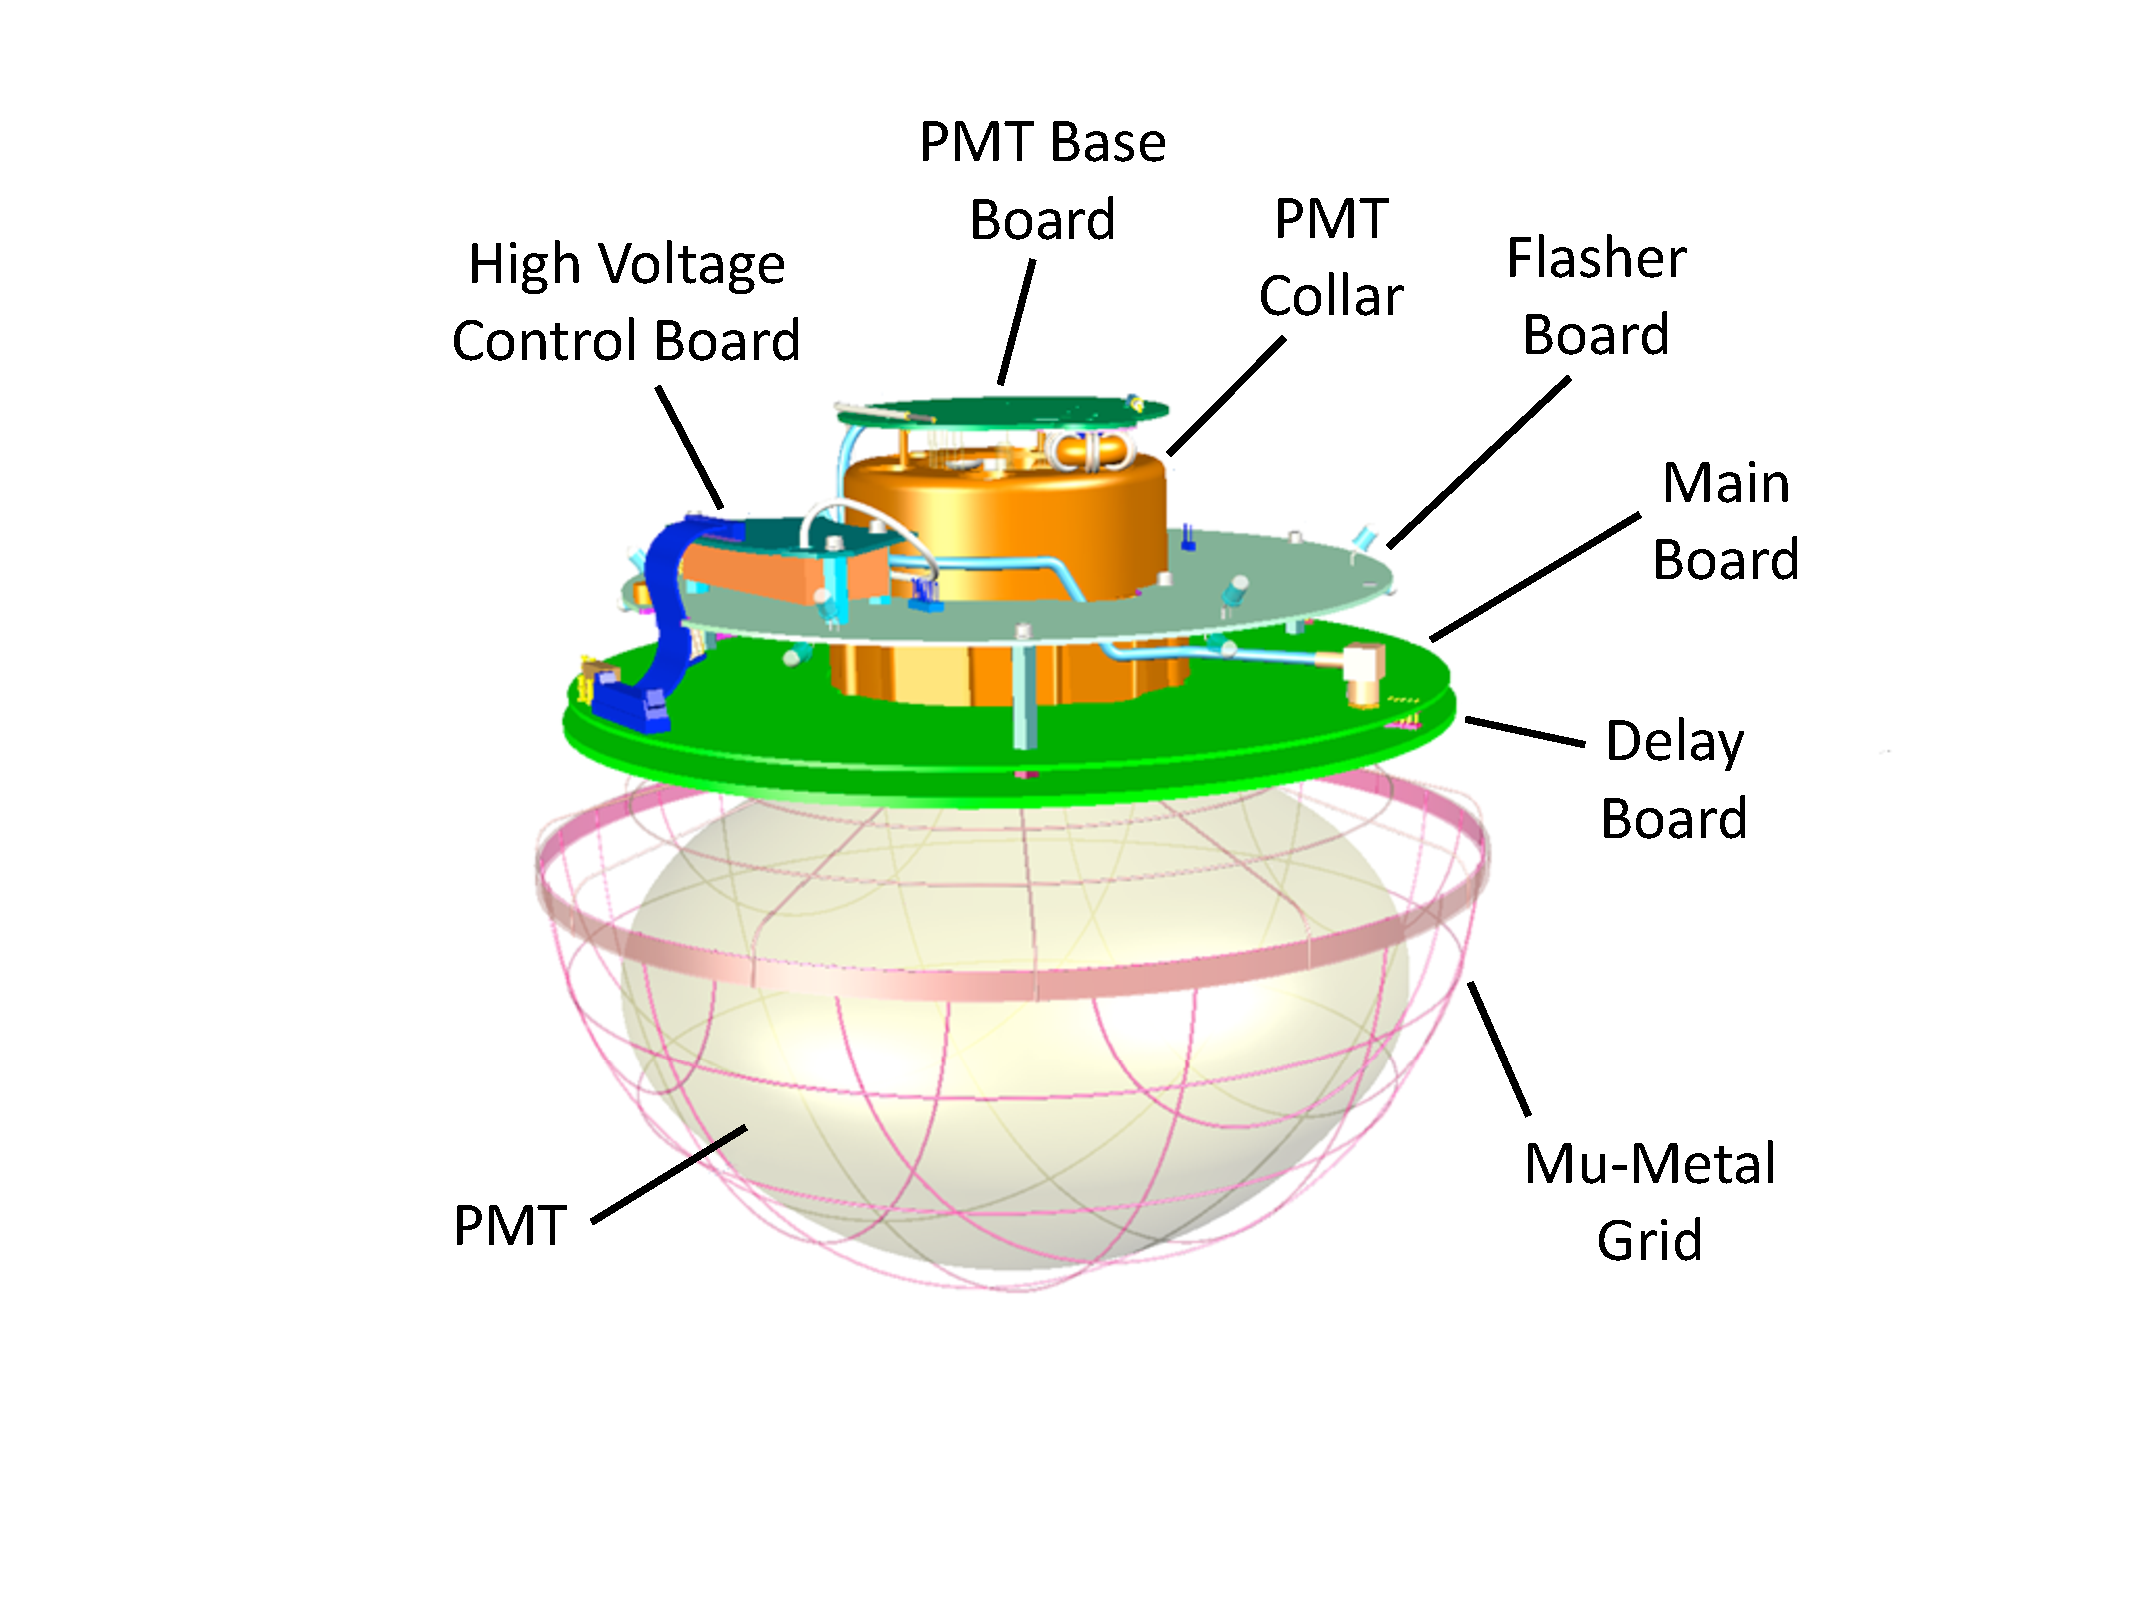
\includegraphics{./figures/nu_in_icecube/domfig1a-DOM3DModel.pdf}
	\caption{A schematic of the DOM, showing its main components \cite{Aartsen_2017}.}
	\labfig{DOM_schematic}
\end{marginfigure}

\begin{description}
    \item[Glass Vessel Properties :] The glass vessel of the DOM is engineered to withstand the extreme pressures found in the deep Antarctic ice. This includes the constant long-term pressure of about 250 bar and the temporary pressure spikes of up to 690 bar experienced during the refreezing process after deployment using a hot water drill. The vessel is composed of two 0.5-inch thick hollow glass hemispheres, which are joined together with optical glue. This design not only provides a robust and hermetic seal to protect the internal electronics but also maintains the optical clarity necessary for the PMT to function effectively. The glass material is chosen for its strength, transparency, and resistance to the harsh conditions in the ice.

    \item[PMT :] The PMT within the DOM is a 10-inch diameter tube that utilizes a box-and-line dynode chain with 10 stages to amplify the faint light signals detected in the ice. The PMTs used in standard in-ice DOMs have a quantum efficiency peaking at 25\% whereas, DeepCore DOMs, designed to detect lower energy neutrinos, feature PMTs with a higher peak quantum efficiency of 34\% near the 390 nm wavelength. These PMTs are operated at a gain of $10^7$.

    \item[Gel :] A high strength, silicon gel is used between the photocathode area and the glass vessel to provide optical coupling and strong mechanical support to the DOM system. This gel has a high optical clarity, with 97\% transmission at 400 nm. It shows no signs of deterioration even after a decade, ensuring reliable performance.

    \item[Magnetic Shield :] The ambient magnetic field at the South Pole, measuring around 550 milligauss (mG), angled 17 degrees from vertical, can significantly affect the performance of the PMT. This includes reducing collection efficiency by 5-10\% and causing gain variations of up to 20\%, depending on the PMT's azimuthal orientation. To mitigate these effects, a mu-metal cage is installed around the PMT bulb, extending up to its neck. This cage is constructed from a mesh of 1 mm diameter wires with a spacing of 66 mm. Although this mesh blocks about 4\% of the incident light, it substantially reduces the adverse impacts of the magnetic field, ensuring more consistent and reliable performance of the PMT.

    \item[PMT Base and High Voltage Boards :] The high voltage board includes a Digital to Analog Converter (DAC) and an Analog to Digital Converter (ADC) for precise control and monitoring of the voltages supplied to the PMT. The high voltage generator on this board provides the necessary power, which is then regulated and distributed by the voltage divider circuits on the PMT base board. These circuits are specifically designed for low power consumption, ensuring efficient and stable operation of the PMT.
    
    \item[Main Board :] The main board serves as the central processing unit (CPU) of the DOM, managing and coordinating all other electronic components. It digitizes the waveforms detected by the PMT, providing a digital representation of the light signals for further analysis. The main board also temporarily stores data, calibrates the internal clock, and exchanges local coincidence information with neighboring DOMs (see \ref{sec:DAQ}). It communicates directly with the Data Acquisition (DAQ) system, ensuring the seamless transfer of data to the IceCube Lab. Additionally, the main board hosts an adjustable low-intensity optical source, which is used to calibrate the PMT's gain and timing, ensuring consistent and accurate performance.
    
    \item[Flasher Board :] Flasher board contains 12 LEDs each having specified output wavelength of $405\pm5 \mathrm{nm}$,
    %  \marginnote{
    %     \begin{kaobox}[title="color DOMs" or CDOMs]
    %         16 of the 5160 \emph{in-ice} DOMs have multi-wavelength LEDs on their Flasher boards. 8 of these DOMs are on string 79 (quite at the centre of the detector, one of the DeepCore strings) and the other 8 on string 14 on the edge of the detector. 
    %     \end{kaobox}}
        which generates lights \emph{in situ} to make various caliberation related measurements. In addition, this board can verify timing responses (useful for many, including analysis presented in this thesis, reconstruction processes). Additionaly, to measure \emph{the optical properties} of the South Pole Ice (see section \ref{sec:icemodel}) and locations of the DOMs in ice.
    
\end{description}

\subsection{Trigger and Data Acquisition}
\label{sec:DAQ}
Ever Since the initial deployment of the first string, the detector has been consistently gathering data, maintaining an average uptime of nearly 99\% \sidecite{Abbasi_2009}. \emph{The photocathode} of the PMT of a DOM, \emph{captures} a photon which then generates \emph{photoelectrons} which are accelerated through the series of 10 dynodes to generate measurable \emph{photocurrent}. This current is integrated over a time to obtain collected charge in units of \emph{photoelectrons or PEs}, through which \emph{photovoltage} is produced at the mainboard, over time, known as \emph{waveform}. These waveforms are then digitized to acquire and relay the data to the Northern Hemisphere.

Depending on how many photons hit the PMT, these waveforms can have different amplitudes ranging from 1mV upto the linearity limit of the PMT (~2 V) in time range of 12-1500 ns. The In Order to access this rather broad dynamic range, the digitiser used, Analog Transient Waveform Digitiser (ATWD) have three channels to amplify the waveform by factor of 0.25, 2 and 16. Moreover, 2 sets of ATWD are used that can operate alternatively in order to reduce the deadtime. ATWD can digitize voltage withinn duration of 427 ns, a window sufficient to reconstruct light produced within 10s of m around a given DOM. Naturally, some photons produced in energetic interactions may travel larger distances, producing faint but detectable waveforms. To amplify and digitize these waveforms, a fast Analog to Digital Converter (fADC) is also used, together ATWD+fADC is reffered as a \emph{DOMLaunch}.

The aforementioned digitization only happens if the voltage threshold of the onboard discriminator is met, which is kept at voltage equivalent to a PE of 0.25, or in other words, a DOM is \emph{hit}. If at least two neighbouring DOMs, on the same string produces individual \emph{hits} within 1 $\mu\mathrm{s}$ called \emph{Hard Local Coincidence(HLC)}, the full \emph{DOMLaunch} is transmitted to the surface. Otherwise, only the timestamp and minimal amplitude/charge information is sent known as \emph{Soft Local Coincidence(SLC)}. The HLC condition helps reduce false triggers from PMT dark noise, which is independent across DOMs. \emph{The Data Acquisition System (DAQ)} processes further uses these HLC hits to look for temporal coincidences. Most commonly used trigger in IceCube is the so-called \emph{The Single Multiplicity Trigger (SMT-8)}, that requires eight or more HLC hits within 5 $\mu\mathrm{s}$ timewindow. If and when SMT8 trigger conditions are met, all launches (HLC and SLC) are combined into what is called an \emph{event}. 

Various algorithms are used to make an estimate of event properties such as direction, deposited energy, morphology etc. The South Pole has limited computational resources, so only simple first guess algorithms can be used there called \emph{online filters}. Processed data is transmitted to the Northern Hemisphere. After this, more sophisticated reconstruction algorithms are applied to reduce and tailor the data as per Physics analysis goal. \todo{cite simulation/reco chapter here}


\section{Optical Properties of the South Pole ice}
The ice at the South Pole is a crucial part of the IceCube detector. It acts as both the detection target and the medium through which light propagates. Unlike the DOM hardware, which has been extensively studied in the laboratory, the glacial ice can only be measured in its actual environment, making it more challenging to describe. Understanding and calibrating this medium well is essential for accurate physics measurements,as it affects the systematic uncertainties in the measurements. The optical properties of the South Pole ice were first studied using ice cores from deep regions below 2000 m, collected from drill sites about 1000 km away from the South Pole. The deep South Pole ice was initially measured with the LED calibration system of AMANDA. Additionally, during the construction of IceCube, dust concentrations in the glacial ice were measured using a dust logger deployed into some drill holes.
\label{sec:icemodel}

